%%
%% MemoryLab (c) 2021-22 Christopher A. Bohn
%%
%% Licensed under the Apache License, Version 2.0 (the "License");
%% you may not use this file except in compliance with the License.
%% You may obtain a copy of the License at
%%     http://www.apache.org/licenses/LICENSE-2.0
%% Unless required by applicable law or agreed to in writing, software
%% distributed under the License is distributed on an "AS IS" BASIS,
%% WITHOUT WARRANTIES OR CONDITIONS OF ANY KIND, either express or implied.
%% See the License for the specific language governing permissions and
%% limitations under the License.
%%

%%
%% (c) 2021 Christopher A. Bohn
%%

\documentclass[12pt]{article}

\usepackage{fullpage}
\usepackage{fancyhdr}
\usepackage[procnames]{listings}
\usepackage{hyperref}
\usepackage{textcomp}
\usepackage{bold-extra}
\usepackage[dvipsnames]{xcolor}
\usepackage{etoolbox}


% Customize the semester (or quarter) and the course number

\newcommand{\courseterm}{Spring 2022}
\newcommand{\coursenumber}{CSCE 231}

% Customize how a typical lab will be managed;
% you can always use \renewcommand for one-offs

\newcommand{\runtimeenvironment}{your account on the \textit{csce.unl.edu} Linux server}
\newcommand{\filesource}{Canvas or {\footnotesize$\sim$}cse231 on \textit{csce.unl.edu}}
\newcommand{\filesubmission}{Canvas}

% These are placeholder commands and will be renewed in each lab

\newcommand{\labnumber}{}
\newcommand{\labname}{Lab \labnumber\ Assignment}
\newcommand{\shortlabname}{}
\newcommand{\duedate}{}

% Individual or team effort

\newcommand{\individualeffort}{This is an individual-effort project. You may discuss concepts and syntax with other students, but you may discuss solutions only with the professor and the TAs. Sharing code with or copying code from another student or the internet is prohibited.}
\newcommand{\teameffort}{This is a team-effort project. You may discuss concepts and syntax with other students, but you may discuss solutions only with your assigned partner(s), the professor, and the TAs. Sharing code with or copying code from a student who is not on your team, or from the internet, is prohibited.}
\newcommand{\freecollaboration}{In addition to the professor and the TAs, you may freely seek help on this assignment from other students.}
\newcommand{\collaborationrules}{}

% Do you care about software engineering?

\providebool{allowspaghetticode}

\setbool{allowspaghetticode}{false}

\newcommand{\softwareengineeringfrontmatter}{
    \ifboolexpe{not bool{allowspaghetticode}}{
        \section*{No Spaghetti Code Allowed}
        In the interest of keeping your code readable, you may \textit{not} use
        any \lstinline{goto} statements, nor may you use any \lstinline{break}
        statements to exit from a loop, nor may you have any functions
        \lstinline{return} from within a loop.
    }{}
}

\newcommand{\spaghetticodepenalties}[1]{
    \ifboolexpe{not bool{allowspaghetticode}}{
        \penaltyitem{1}{for each \lstinline{goto} statement, \lstinline{break}
            statement used to exit from a loop, or \lstinline{return} statement
            that occurs within a loop.}
    }{}
}

% You shouldn't need to customize these,
% but you can if you like

\lstset{language=C, tabsize=4, upquote=true, basicstyle=\ttfamily}
\newcommand{\function}[1]{\textbf{\lstinline{#1}}}
\setlength{\headsep}{0.7cm}
\hypersetup{colorlinks=true}

\newcommand{\startdocument}{
    \pagestyle{fancy}
    \fancyhf{}
    \lhead{\coursenumber}
    \chead{\ Lab \labnumber: \labname}
    \rhead{\courseterm}
    \cfoot{\shortlabname-\thepage}

	\begin{document}
	\title{\ Lab \labnumber}
	\author{\labname}
	\date{Due: \duedate}
	\maketitle

    \textit{\collaborationrules}
}

\newcommand{\rubricitem}[2]{\item[\underline{\hspace{1cm}} +#1] #2}
\newcommand{\bonusitem}[2]{\item[\underline{\hspace{1cm}} Bonus +#1] #2}
\newcommand{\penaltyitem}[2]{\item[\underline{\hspace{1cm}} -#1] #2}

%%
%% labs/common/semester.tex
%% (c) 2021-22 Christopher A. Bohn
%%
%% Licensed under the Apache License, Version 2.0 (the "License");
%% you may not use this file except in compliance with the License.
%% You may obtain a copy of the License at
%%     http://www.apache.org/licenses/LICENSE-2.0
%% Unless required by applicable law or agreed to in writing, software
%% distributed under the License is distributed on an "AS IS" BASIS,
%% WITHOUT WARRANTIES OR CONDITIONS OF ANY KIND, either express or implied.
%% See the License for the specific language governing permissions and
%% limitations under the License.
%%


% Customize the semester (or quarter) and the course number

\newcommand{\courseterm}{Fall 2022}
\newcommand{\coursenumber}{CSCE 231}

% Customize how a typical lab will be managed;
% you can always use \renewcommand for one-offs

\newcommand{\runtimeenvironment}{your account on the \textit{csce.unl.edu} Linux server}
\newcommand{\filesource}{Canvas or {\footnotesize$\sim$}cse231 on \textit{csce.unl.edu}}
\newcommand{\filesubmission}{Canvas}

% Customize for the I/O lab hardware

\newcommand{\developmentboard}{Arduino Nano}
%\newcommand{\serialprotocol}{SPI}
\newcommand{\serialprotocol}{I2C}
%\newcommand{\displaymodule}{MAX7219digits}
%\newcommand{\displaymodule}{MAX7219matrix}
\newcommand{\displaymodule}{LCD1602}

\setbool{usedisplayfont}{true}

\newcommand{\obtaininghardware}{
    The EE Shop has prepared ``class kits'' for CSCE 231; your class kit costs \$30.
    The EE Shop is located at 122 Scott Engineering Center and is open M-F 7am-4pm. You do not need an appointment.
    You may pay at the window with cash, with a personal check, or with your NCard.
    The EE shop does \textit{not} accept credit cards.
}

% Update to reflect the CS2 course(s) at your institute

\newcommand{\cstwo}{CSCE~156, RAIK~184H, or SOFT~161}

% Do you care about software engineering?

\setbool{allowspaghetticode}{false}

% Which assignments are you using this semester, and when are they due?

\newcommand{\pokerlabnumber}{1}
\newcommand{\pokerlabcollaboration}{
    Sections~\ref{sec:connecting}, \ref{sec:terminology}, \ref{sec:gettingstarted}, \ref{subsec:typesofpokerhands}, and~\ref{subsec:studythecode}: \freecollaboration
    Sections~\ref{sec:completingcard} and~\ref{subsec:completepoker}: \individualeffort
}
\newcommand{\pokerlabdue}{Week of August 29, before the start of your lab section}

\newcommand{\keyboardlabnumber}{2}
\newcommand{\keyboardlabcollaboration}{\individualeffort}
\newcommand{\keyboardlabdue}{Week of January 31, before the start of your lab section}

\newcommand{\pointerlabnumber}{3}
\newcommand{\pointerlabcollaboration}{\individualeffort}
\newcommand{\pointerlabdue}{Week of February 7, before the start of your lab section}

\newcommand{\integerlabnumber}{4}
\newcommand{\integerlabcollaboration}{\individualeffort}
\newcommand{\integerlabdue}{Week of February 14, before the start of your lab section}

\newcommand{\floatlabnumber}{5}
\newcommand{\floatlabcollaboration}{\individualeffort}
\newcommand{\floatlabdue}{soon}

\newcommand{\addressinglabnumber}{6}
\newcommand{\addressinglabcollaboration}{\individualeffort}
\newcommand{\addressinglabdue}{Week of February 28, before the start of your lab section}

%bomblab was 7
%attacklab was 8

\newcommand{\pollinglabnumber}{9}
\newcommand{\pollinglabcollaboration}{\individualeffort}
\newcommand{\pollinglabdue}{Week of April 11, before the start of your lab section}
\newcommand{\pollinglabenvironment}{your \developmentboard-based class hardware kit}

\newcommand{\ioprelabnumber}{\pollinglabnumber-prelab}
\newcommand{\ioprelabcollaboration}{\freecollaboration}
\newcommand{\ioprelabdue}{Before the start of your lab section on April 5 or 6}

\newcommand{\interruptlabnumber}{10}
\newcommand{\interruptlabcollaboration}{\individualeffort}
\newcommand{\interruptlabdue}{Week of April 18, before the start of your lab section}
\newcommand{\interruptlabenvironment}{your \developmentboard-based class hardware kit}

\newcommand{\capstonelab}{ComboLock}    % this will come into play when we generalize capstonelab
\newcommand{\capstonelabnumber}{11}
\newcommand{\capstonelabcollaboration}{\teameffort}
\newcommand{\capstonelabdue}{Week of May 2, Before the start of your lab section\footnote{See Piazza for the due dates of teams with students from different lab sections.}}
\newcommand{\capstonelabenvironment}{your \developmentboard-based class hardware kit}

\newcommand{\memorylabnumber}{12}
\newcommand{\memorylabcollaboration}{This is an individual-effort project. You may discuss the nature of memory technologies and of memory hierarchies with classmates, but you must draw your own conclusions.}
\newcommand{\memorylabdue}{Week of May 2, at the end of your lab section}
\newcommand{\memorylabenvironment}{your \developmentboard-based class hardware kit and your account on the \textit{csce.unl.edu} Linux server}

% Labs not used this semester

\newcommand{\concurrencylabnumber}{XX}
\newcommand{\concurrencylabcollaboration}{\individualeffort}
\newcommand{\concurrencylabdue}{not this semester}

\newcommand{\ssbcwarmupnumber}{XX}
\newcommand{\ssbcwarmupcollaboration}{\freecollaboration}
\newcommand{\ssbcwarmupdue}{not this semester}

\newcommand{\ssbcpollingnumber}{XX}
\newcommand{\ssbcpollingcollaboration}{\individualeffort}
\newcommand{\ssbcpollingdue}{not this semester}

\newcommand{\ssbcinterruptnumber}{XX}
\newcommand{\ssbcinterruptcollaboration}{\individualeffort}
\newcommand{\ssbcinterruptdue}{not this semester}


\usepackage{graphicx}

%%% StickyNote from https://tex.stackexchange.com/questions/159679/sticky-notes-image
\usepackage{xparse}
% \usepackage{fontspec}
% \setmainfont{Humor Sans}
\usepackage{tikz}
\usetikzlibrary{shadows}
\usepackage{lipsum}\usepackage{array,color,colortbl}
\definecolor{LightGreen}{rgb}{0.88,1,0.88}

\definecolor{myyellow}{RGB}{242,226,149}

\NewDocumentCommand\StickyNote{O{6cm}mO{6cm}}{%
\begin{tikzpicture}
\node[
drop shadow={
  shadow xshift=2pt,
  shadow yshift=-4pt
},
inner xsep=7pt,
fill=myyellow,
xslant=-0.1,
yslant=0.1,
inner ysep=10pt
] {\parbox[t][#1][c]{#3}{#2}};
\end{tikzpicture}%
}
%%%

\renewcommand{\labnumber}{\memorylabnumber}
\renewcommand{\labname}{Memory Measurement Lab}
\renewcommand{\shortlabname}{memorylab}
\renewcommand{\collaborationrules}{\memorylabcollaboration}
\renewcommand{\duedate}{\memorylabdue}
\newcommand{\nano}{\developmentboard} % TODO: replace \nano with \developmentboard
\renewcommand{\runtimeenvironment}{\memorylabenvironment}
\pagelayout
\begin{document}
\labidentifier


In this assignment, you will measure the speed of different memories and draw
conclusions based on your understanding of memory hierarchies. \textbf{You will
be able to complete this lab assignment during lab time.}

The instructions are written assuming you will run the code on
\runtimeenvironment.

\section*{Learning Objectives}

After successful completion of this assignment, students will be able to:
\begin{itemize}
\item Identify the relative speeds of some types of memory.
\item Draw conclusions about a cache's design based on timing data.
\item Recognize the performance benefits of cache-friendly code.
\end{itemize}

\subsection*{Continuing Forward}

This final lab assignment should give you a qualitative appreciation of memory
concepts discussed in the course.

\section*{During Lab Time}

\textbf{You must complete this lab assignment during lab time}; it is due at the
end of your scheduled lab session. The TAs will be available to answer
questions.

\section{Scenario}

{\large \textbf{Mid-Credits Scene}:} Herb walks up to you. ``Could you do me a
favor, please? I'd like to better characterize some of the performance
characteristics of the Cow Pi, but I don't have the time to do so. Now that the
urgency over developing the security systems is behind us, I need to get back to
Eclectic Electronics to clean up a couple of messes that I had to leave there
while we developed the Cow Pi. Do you mind measuring the memory performance?''

\section{Arduino Memories}

The ATmega328P microcontroller on your \nano\ has three memories:
\begin{itemize}
\item 2KB SRAM data memory
\item 1KB EEPROM data memory
\item 32KB flash instruction memory
\end{itemize}

Unlike modern microprocessors, microcontrollers typically don't have cache
memories because the CPU and memory speeds are well-matched (for example,
the ATmega328P on your \nano\ is clocked at 16MHz, about two orders of
magnitude slower than the microprocessor in your personal computer).

The instruction memory is designed to deliver instructions quickly, given the
predictable access pattern for instruction fetches. This allows the CPU in the
ATmega328P to have a 2-stage pipeline, as shown in Figure~\ref{fig:pipelining}.
It is possible to place read-only data in the flash
memory;\footnote{\url{https://www.nongnu.org/avr-libc/user-manual/pgmspace.html}}$^,$\footnote{\url{https://www.nongnu.org/avr-libc/user-manual/pgmspace_8h.html}}
however, random accesses to the flash memory will require more than the one
clock cycle that instruction fetches enjoy. (Similarly, read-only data can be
placed in the EEPROM,\footnote{\url{https://www.nongnu.org/avr-libc/user-manual/group__avr__eeprom.html}}
but we will not measure the EEPROM's performance in this lab assignment.)

\begin{figure}
    \centering
    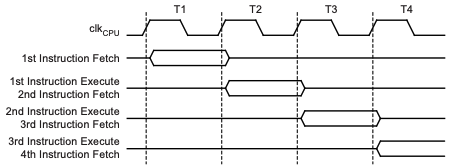
\includegraphics[width=10cm]{ATmega328P_PipelineTiming}
    \caption{Pipelined instruction fetches and instruction executions. \tiny Copied from ATmega328P Data Sheet, Figure~6-4 \label{fig:pipelining}}
\end{figure}

\subsection{MemoryMeasurement.ino / MemoryManagement.cpp}

Open \textit{MemoryMeasurement.ino} in the Arduino IDE or \textit{MemoryMeasurement.cpp} in VS~Code. The program takes four
measurements. The \function{get_baseline_time()} function performs every
calculation made by the remaining functions \textit{except} for the data
retrievals that are unique to each of the remaining functions. The time
required for this calculations will be subtracted from the times required for
the other functions, allowing us to calculate the time required to retrieve
data. The \function{time_register_access()} function retrieves values from the
CPU's general-purpose registers. The \function{time_sram_access()} function
retrieves values from the microcontroller's SRAM memory. Finally,
\function{time_flash_access()} retrieves values from the microcontroller's
flash memory.

After you upload the sketch to your \nano, those four functions will each run
once, and the average time to read a value from a CPU register, from SRAM, and
from flash memory will be calculated and displayed. If you wish to re-run the
sketch, you can press the \nano's RESET button to restart the program without
re-uploading it.

Upload \textit{MemoryMeasurement} to your \nano\ now.

\vspace{.5cm}

Open the \textit{answers.txt} file in a text editor.

\subsection{Data in CPU Registers}

To draw conclusions about reading data in the CPU's general-purpose registers,
two additional pieces of information will be useful. First, calculate the CPU
clock's period. Because the clock frequency is 16MHz, you can calculate its
period, in microseconds (µs), by dividing $1 \div 16$. Do so and record your
answer in \textit{answers.txt}.

Next, note in Figure~\ref{fig:AluTiming} that retrieving values from
the CPU registers is part of the CPU's ``execute'' stage.

\begin{figure}
    \centering
    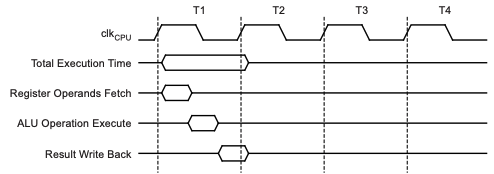
\includegraphics[width=10cm]{ATmega328P_AluTiming}
    \caption{Timing within ATmega328P's ``execute'' stage. \tiny Copied from ATmega328P Data Sheet, Figure~6-5 \label{fig:AluTiming}}
\end{figure}

Record in \textit{answers.txt} the amount of time that
\textit{MemoryMeasurement} reports is needed to access data in a CPU
register. What can you conclude about the time required to access data in a CPU
register? Is the reported time significant? Record your answer in
\textit{answers.txt}.

\subsection{Data in SRAM}

Record in \textit{answers.txt} the amount of time that
\textit{MemoryMeasurement}  reports is needed to access data in a SRAM.

Notice in Figure~\ref{fig:SramTiming} that the ATmega328P Data Sheet states
that accessing data in SRAM requires two clock cycles. Is the reported time to
access data in SRAM consistent with the data sheet? Why or why not? Record your
answers in \textit{answers.txt}.

\begin{figure}
    \centering
    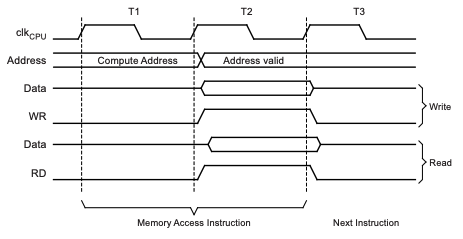
\includegraphics[width=10cm]{ATmega328P_SramTiming}
    \caption{Timing of SRAM Access on the ATmega328P. \tiny Copied from ATmega328P Data Sheet, Figure~7-3 \label{fig:SramTiming}}
\end{figure}

\subsection{Data in Flash Memory}

Record in \textit{answers.txt} the amount of time that
\textit{MemoryMeasurement} reports is needed to access data in a flash
memory.

The ATmega328P Data Sheet does not describe timing of accesses to flash memory
except for instruction fetches, but you can draw conclusions based on the
measurements taken.

Approximately how many clock cycles are required to read data from flash
memory, according to \textit{MemoryMeasurement}? What conclusions can you
draw about the speed of flash memory relative to the speed of SRAM? Record your
answers in \textit{answers.txt}.

\section{AMD EPYC Caches}

We will now take measurements of the cache memories of the microprocessors on
\textit{cse-linux-01.unl.edu}. Upload \textit{CacheMeasurement.c} to your account on
\textit{cse-linux-01.unl.edu}. Compile it with:

\texttt{gcc -O0 -Wall -o CacheMeasurement CacheMeasurement.c}

You will see two warnings:
\begin{verbatim}
CacheMeasurement.c: In function ‘measure_helper’:
CacheMeasurement.c:68:13: warning: variable ‘datum’ set but not used [-Wunused-but-set-variable]
     uint8_t datum;
             ^~~~~
CacheMeasurement.c: In function ‘measure_cache_lines’:
CacheMeasurement.c:111:22: warning: variable ‘datum’ set but not used [-Wunused-but-set-variable]
     register uint8_t datum;
                      ^~~~~
\end{verbatim}

Normally you should correct your code to address warnings; however, in this
particular case, we are intentionally updating these variables without using
the values they contain.

Open \textit{CacheCharts.xlsx}.

\subsection{Measuring Cache Level Sizes}

Run the program: \texttt{./CacheMeasurement} on \textit{cse-linux-01.unl.edu}. You will
be presented with three options:

\begin{verbatim}
  1. Measure the sizes of cache levels
  2. Determine the size of a cache line
  3. Exit program
Please choose the measurement you wish to take:
\end{verbatim}

For this part of the lab we will use the first option to attempt to discern the
sizes of the different cache levels.

Recall that there are three types of cache misses: Cold (or compulsory) misses,
in which we can replace an invalid cache block with a valid cache block;
Conflict misses, in which a valid cache block must be displaced to allow
another cache block to be placed in the cache even though a different cache
design might have prevented the conflict; and Capacity misses, in which the
working set is too great to fit in the cache, and no cache design could have
prevented a conflict. \textit{CacheMeasurement}'s first option will increase the
working set size until it is too great to fit in the L1 cache, and then until it
is too great to fit in the L2 cache, and finally until it is too great to fit in
the L3 cache. The program will measure how much CPU time your process spends
waiting for data (it will only measure the time allotted to \textit{your}
process, so other process running should have little effect on your
measurements). We are less concerned with the specific amount of time, as we are
with when there are noticeable increases in the time.

Figure~\ref{fig:LaptopCache} shows a graph similar to the one you will
produce. The figure shows the cache size measurements for an Intel Core i7
processor in a 2018 MacBook Pro. This particular processor has a 32KB L1 data
cache (also a 32KB L1 instruction cache), a 256KB L2 cache, and a 2MB L3 cache.
There are labels showing where these limits are exceeded -- other measurement
artifacts make it difficult to discern the limit of the L1 cache, but we can use
the chart to reasonably estimate the sizes of the L2 and L3 caches with an error
less than a factor of 2.

\begin{figure}
    \centering
    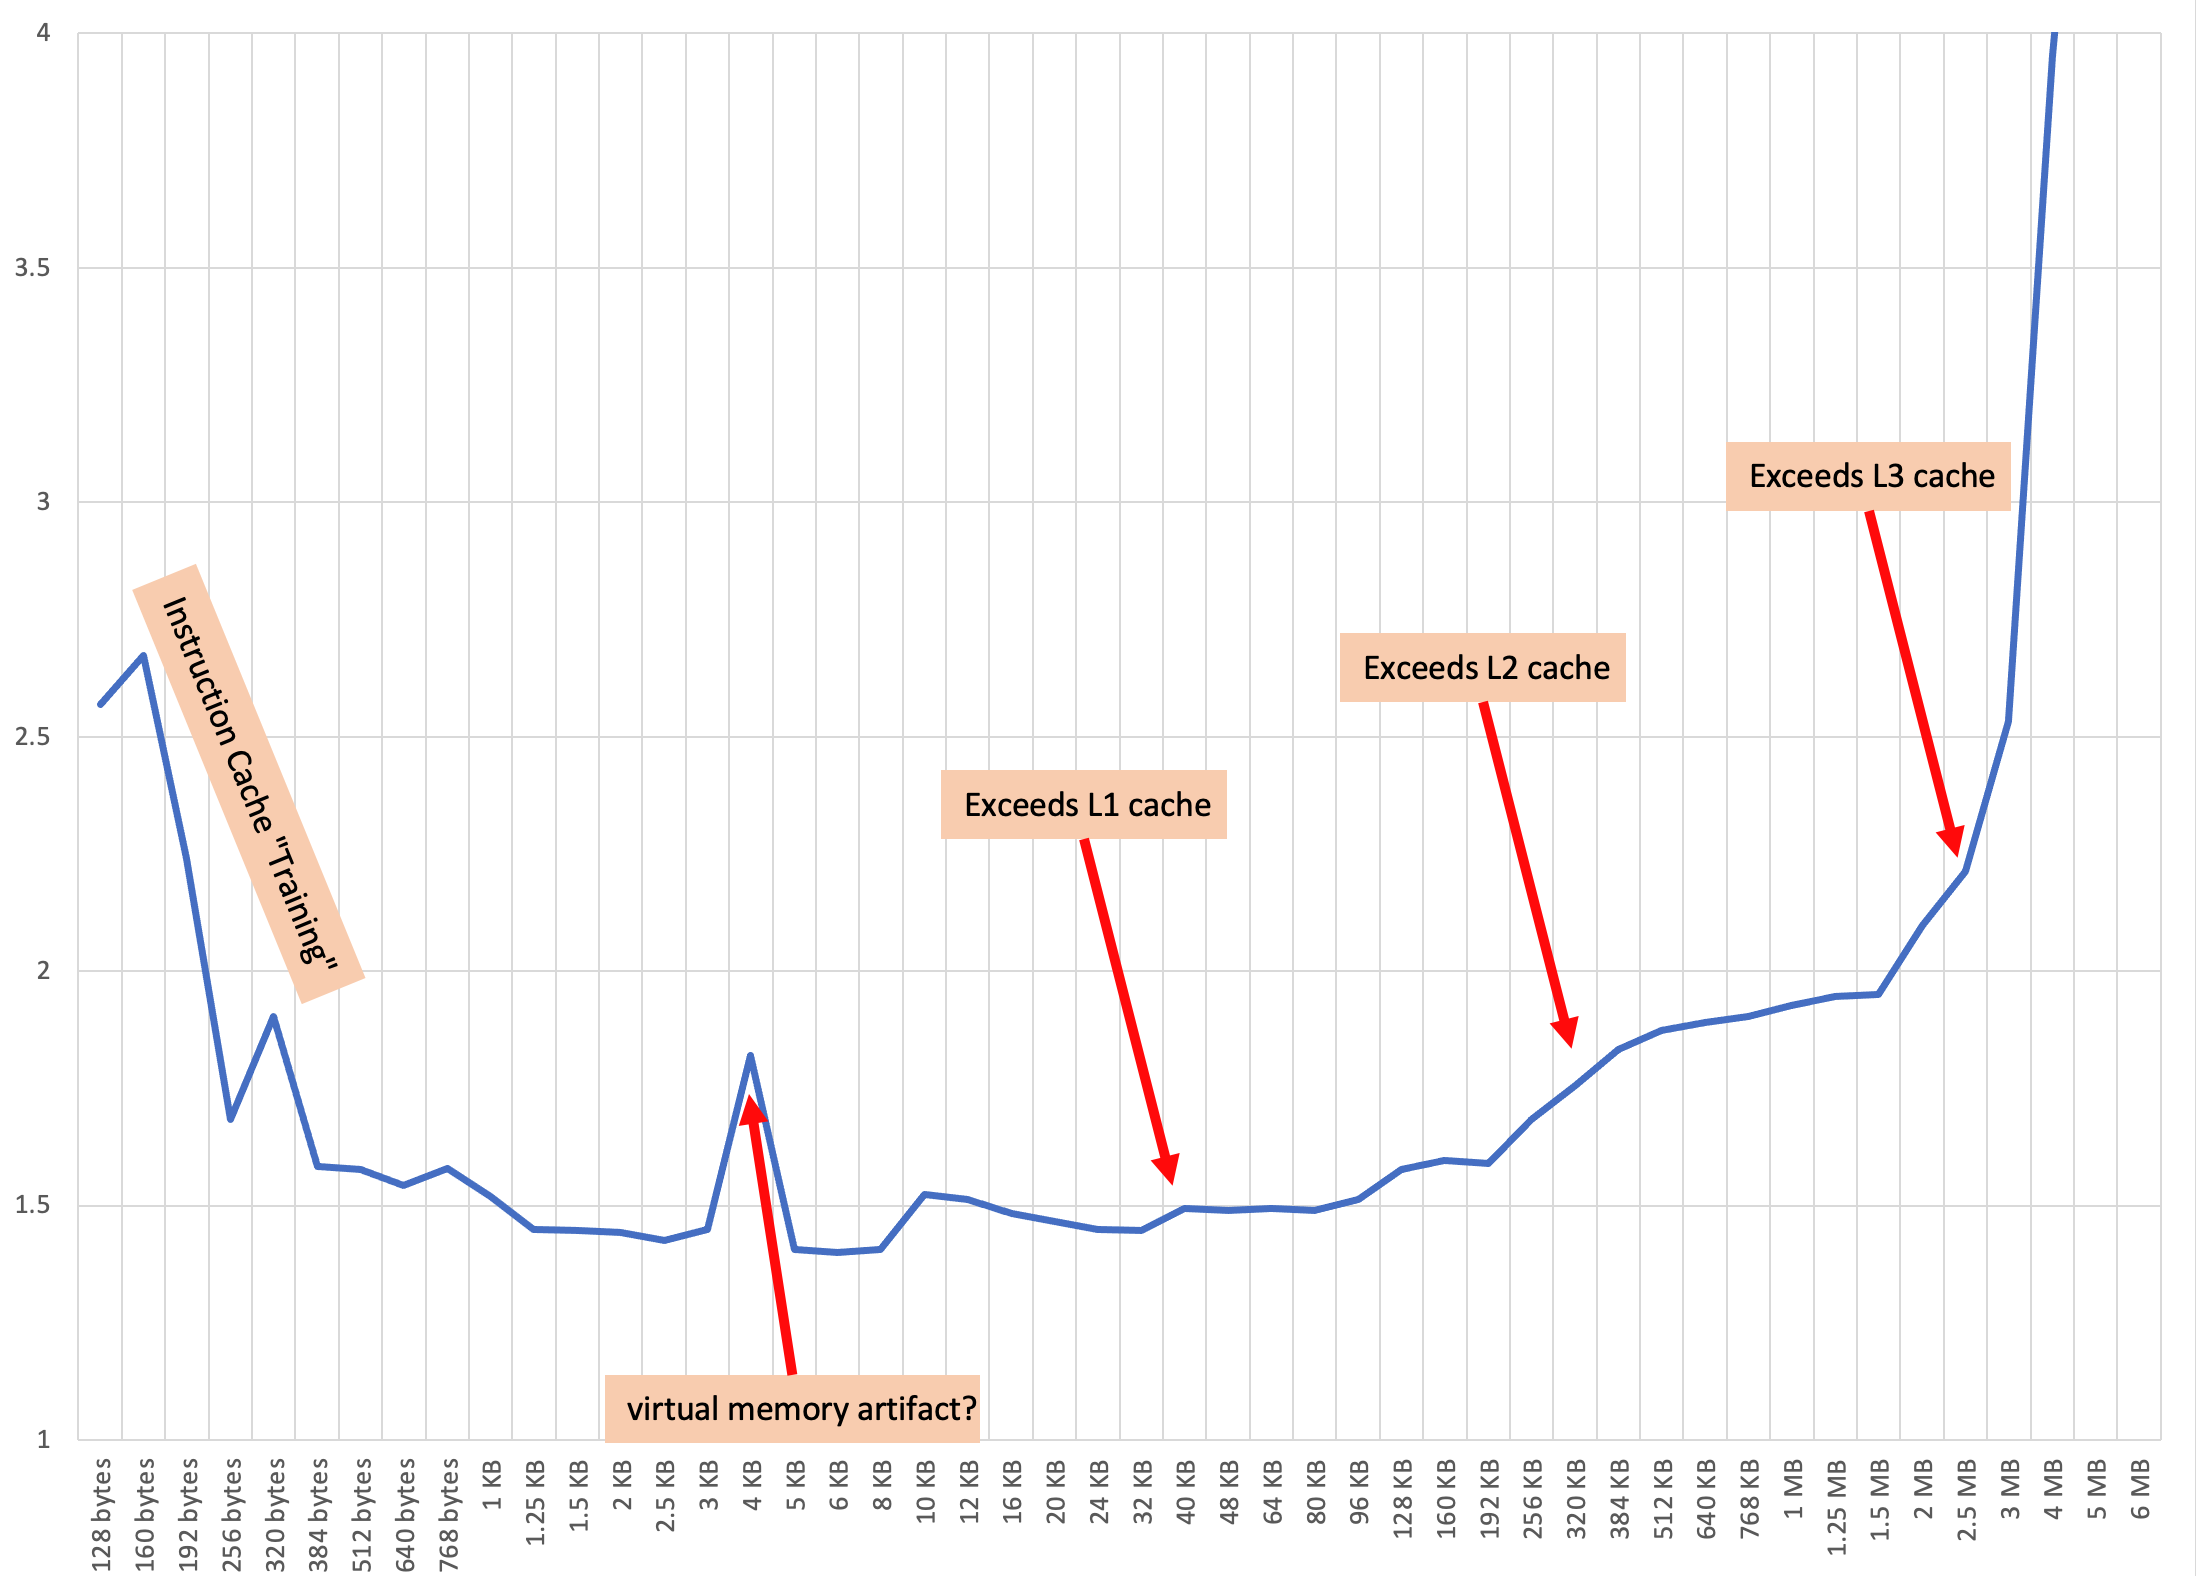
\includegraphics[width=13cm]{IntelI7caches}
    \caption{Measurement of cache levels on Intel Core i7 processor. \label{fig:LaptopCache}}
\end{figure}

Select the first option, and measure the sizes of the cache levels. Copy the
timing data into the ``Data'' tab in \textit{CacheCharts.xlsx}, in cells C2:C52
(that is, under the heading ``first run''). Repeat the first option, copying
the timing data under the ``second run'' heading. Repeat again for a third,
fourth, and fifth run. (If you get the error ``\texttt{Cputime limit exceeded
(core dumped)}'' then restart the program.) Save \textit{CacheCharts.xlsx}.

The ``AVERAGE TIME'' column throws out the longest and shortest measurements
and then averages the remaining three measurements. These averages are plotted
in the ``Cache Size'' tab.

The points at which the working set exceeds the sizes of the L1 and L2 caches
should be fairly distinct. Because the L3 cache is shared among 24 cores, other
processes (as well as other timing artifacts) will likely result in the L3
cache not having a smooth ``plateau'' like the i7 processor has in
Figure~\ref{fig:LaptopCache}.

If there isn't a place on the chart where the timing exceeds the chart's scale,
consider editing \textit{CacheMeasurement.c} to use a greater
\lstinline{MAX_WORKING_SET_SIZE}, re-compiling, and re-running the measurements.

Based on the chart, estimate the sizes of the L1, L2, and L3 caches for the
EPYC processor in \textit{cse-linux-01.unl.edu}. Place your estimates in
\textit{answers.txt}.

\subsection{Measuring Cache Line Size}

For this part of the lab we will use the second option to attempt to discern the
size of a cache line in the EPYC's cache design.

Recall that caches are designed to take advantage of locality, and when memory
access patterns don't take advantage of locality then performance suffers. Your
next set of measurements will exploit this fact by increasing the access stride
so that you can notice when there is a slight increase in timing due to the
stride exceeding the length of a cache line.

Select the second option to determine the size of a cache line. Copy the data
into \textit{CacheChart.xlsx}'s ``Data'' tab, cells C64:C74 (that is, under the
heading ``first run''). Repeat the first option, copying the timing data under
the ``second run'' heading. Repeat again for a third, fourth, and fifth run.
Save \textit{CacheCharts.xlsx}.

The ``AVERAGE TIME'' column throws out the longest and shortest measurements
and then averages the remaining three measurements. These averages are plotted
in the ``Cache Line Size'' tab.

If you can discern a point at which the stride exceeds a cache line, then
estimate the size of a cache line on the AMD EPYC processor, and place your
estimate in \textit{answers.txt}. It's very possible that you won't be able to
do so. If you cannot, then use Figure~\ref{fig:LaptopCacheLine} to estimate the
size of a cache line on the Intel Core i7 processor, and place your estimate in
\textit{answers.txt}.

\begin{figure}
    \centering
    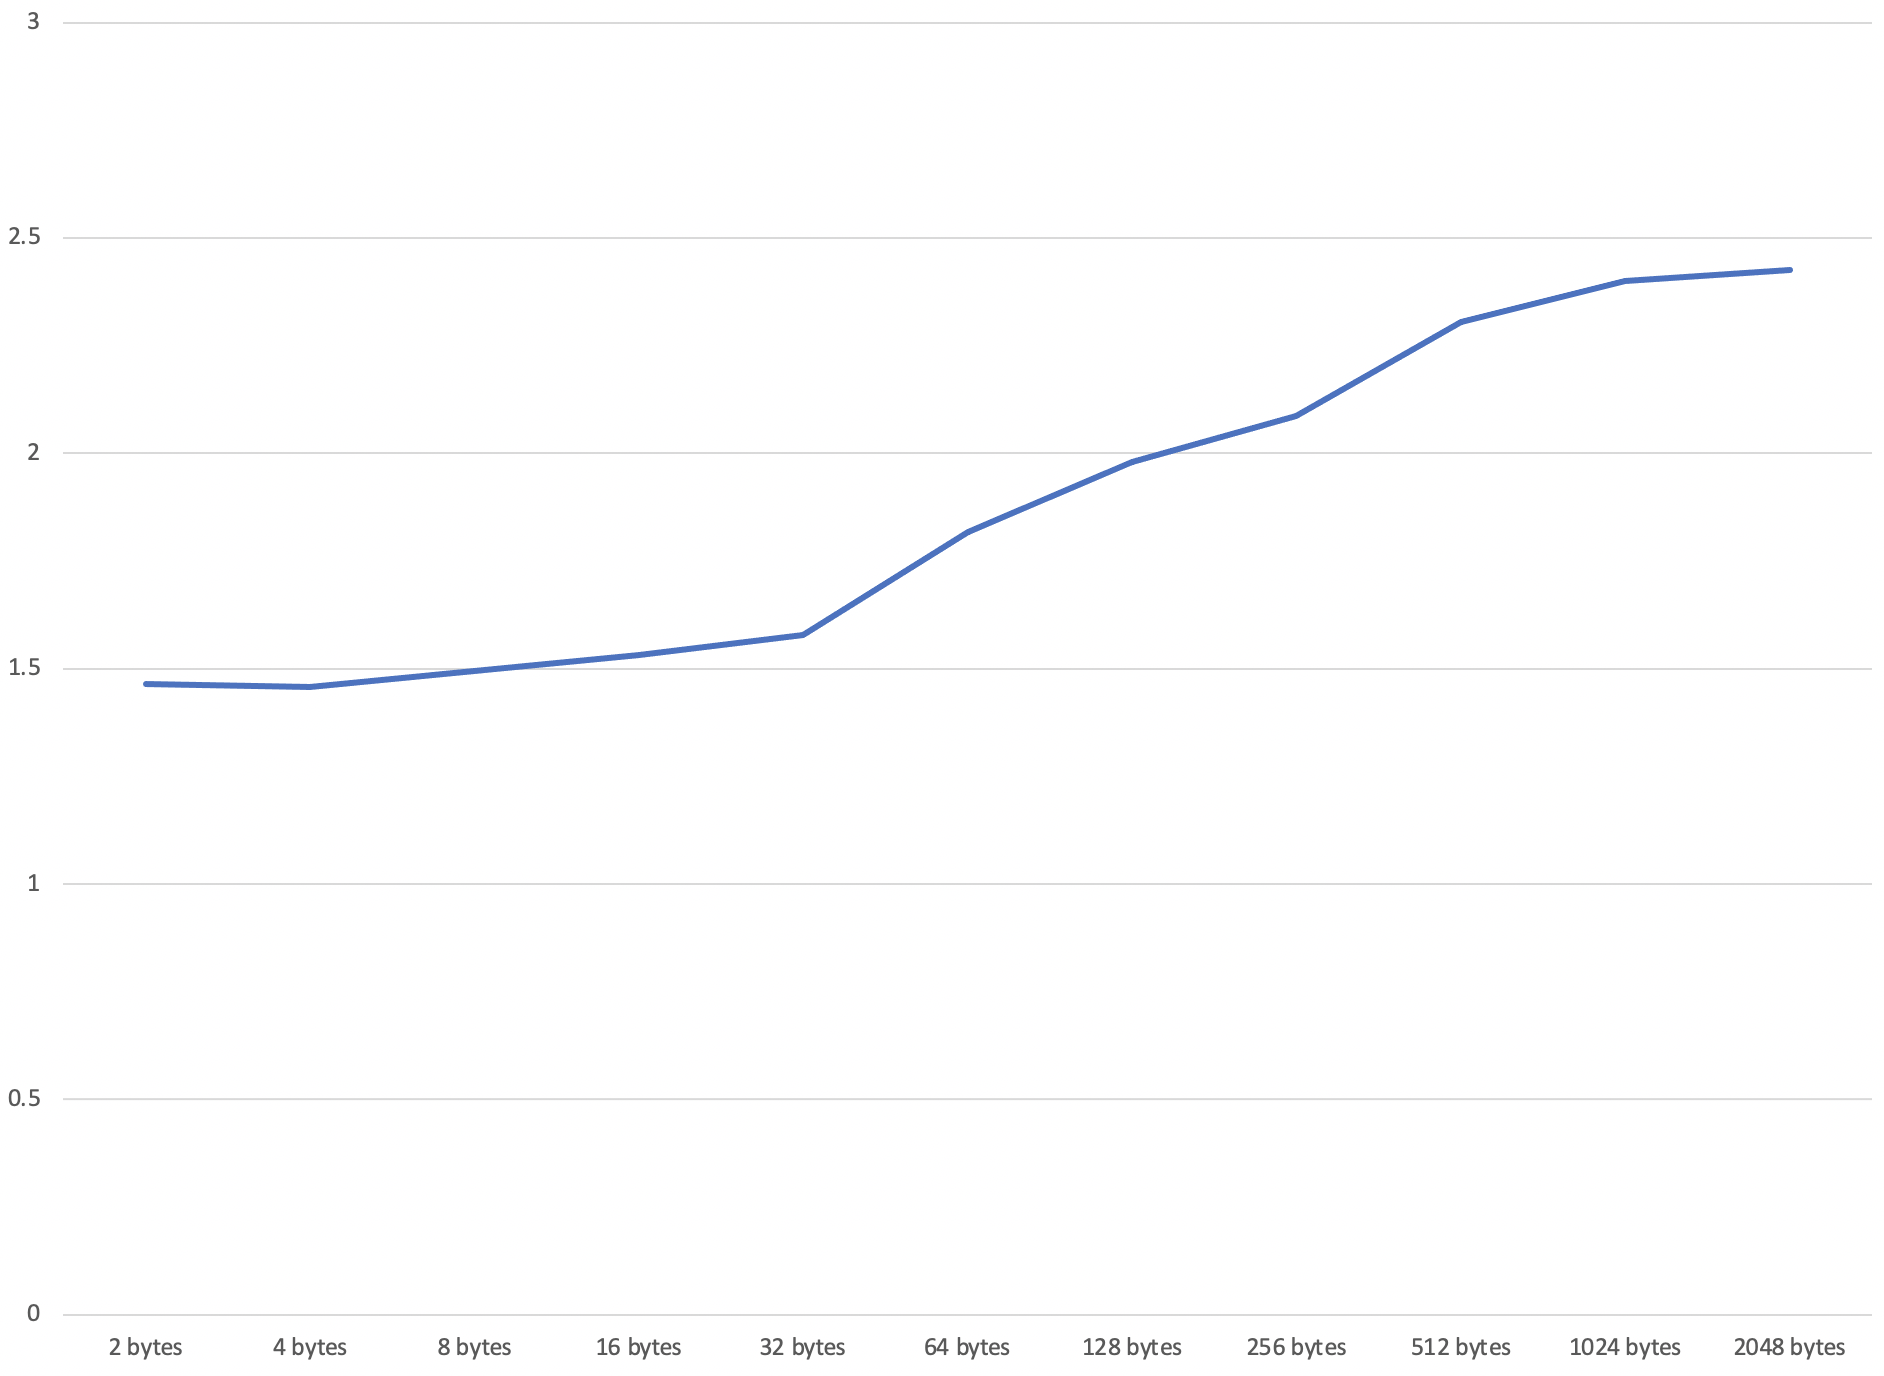
\includegraphics[width=13cm]{IntelI7cacheLine}
    \caption{Measurement of cache lines on Intel Core i7 processor. \label{fig:LaptopCacheLine}}
\end{figure}

\section*{Turn-in and Grading}

When you have completed this assignment, upload \textit{answers.txt} and
\textit{CacheCharts.xlsx} to \filesubmission.

This assignment is worth 10 points. \\

\begin{description}
\rubricitem{1}{Drawing a reasonable conclusion about the time required to
    access data in a CPU register.}
\rubricitem{2}{Concluding whether or not the time to access data in SRAM is
    consistent with the ATmega328P Data Sheet and justifying your conclusion.}
\rubricitem{2}{Drawing a reasonable conclusion about the speed of flash memory
    relative to the speed of SRAM.}
\rubricitem{1}{Measuring the cache level sizes and the cache line size on the
    AMD EPYC processor.}
\rubricitem{2}{Drawing reasonable conclusions about the sizes of the EPYC's L1, L2, and L3 caches.}
\rubricitem{2}{Drawing a reasonable conclusion about the size of the EPYC's cache line, or about the size of the Intel Core i7's cache line.}
\end{description}

Your conclusions do not need to be correct to receive full credit. You can
receive full credit if your conclusions are reasonable, given your measurements.



\section*{Epilogue}

{\large \textbf{Post-Credits Scene}:} As an opportunity to stretch your legs,
you decided to walk from your office at the Pleistocene Petting Zoo to Eclectic
Electronics to personally give Herb your memory measurement data. As you
approach Eclectic Electronics' labs, you notice that the lights are flickering,
and sparks are dripping from the ceiling. You see that a new Cow Pi-based
electronic lock is still holding the lab door shut squarely in its frame -- but
the door frame has been torn from the wall and is laying askew in the hallway.
On the floor is a Cow Pi-based calculator; the display reads: \\
\begin{tabular}{>{\raggedleft}p{3.5cm}>{\raggedleft\arraybackslash}p{1cm}}
    \rowcolor{LightGreen}\display{Robot Count:\phantom{xxxx}} & \display{12} \\
    \rowcolor{LightGreen}\display{-} & \display{1}
\end{tabular}


Peeking into the lab, you see a platform, empty except for a note. The note says:

\begin{center}\StickyNote[5cm]{\begin{center}
i\textsc{Suck \\ Robot Vacuum Cleaner \\ \phantom{x}}
\end{center}\begin{flushleft}
CAUTION! Stuck in ``Malevolent Sentience'' mode. \\ \phantom{x} \\
Do \underline{\underline{not}} turn on until after
troubleshooting the problem and uploading new software.
\end{flushleft}}[7cm]\end{center}

A Cow-Pi based motion alarm chirps as something enters its detection range.

\textit{Cut to black.}

\end{document}
